\documentclass{beamer}
\usetheme{Madrid}
\usecolortheme{seahorse}
\usepackage{graphicx}

\title{Resultados del Analisis de Centralidad}
\author{Equipo de Analisis de Redes}
\date{\today}

\begin{document}

\begin{frame}{1. Resultados interesantes del reporte}
\begin{columns}[T]
\column{0.56\textwidth}
\small
\begin{itemize}
    \item En el informe: 4039 nodos, 88234 aristas y 1 componente conectado (100\%).
    \item \textbf{Densidad 0.0108}: de cada 100 conexiones posibles, solo ~1 existe (red poco densa).
    \item \textbf{Diametro 8}: el camino mas largo entre dos personas es de 8 saltos.
    \item \textbf{Clustering alto}: hay grupos de amigos muy conectados entre si.
    \item El nodo 107 aparece primero en los 3 rankings: es el actor mas influyente del informe.
\end{itemize}
\column{0.44\textwidth}
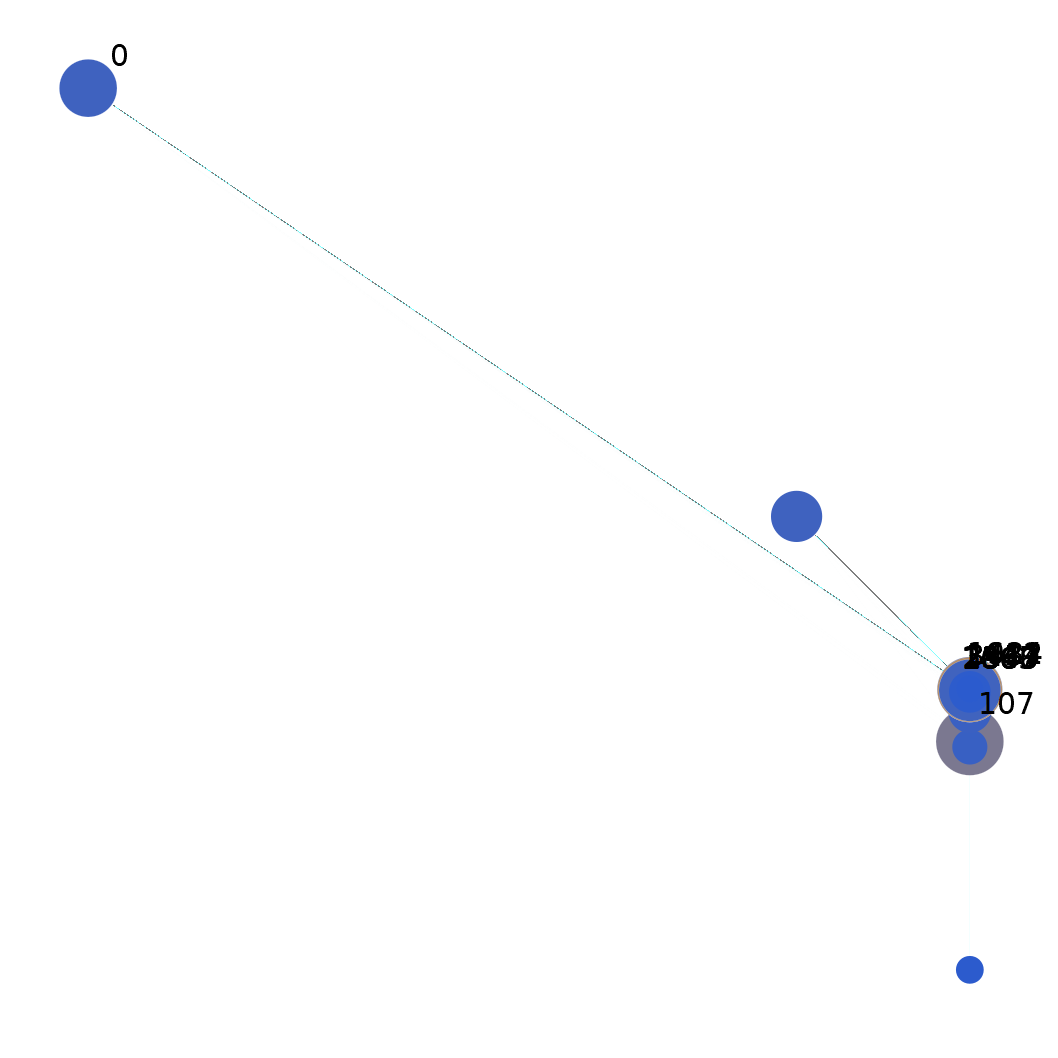
\includegraphics[width=\linewidth]{plots/facebook_red_completa_cairo.png}
\vspace{0.05cm}
{\tiny El tamano del nodo refleja su grado, el color resume su nivel de insercion en el nucleo. Solo se etiquetan los 10 nodos mas populares.}
\end{columns}
\end{frame}

\begin{frame}{2. Inconsistencias encontradas en el reporte}
\begin{columns}[T]
\column{0.56\textwidth}
\scriptsize
\begin{itemize}
    \item \textbf{Nodo 107 lidera las 3 metricas}: degree, betweenness y closeness raramente coinciden. El informe lo reporta pero no lo cuestiona ni lo explica.
    \item \textbf{Assortativity 0.0636 como ``tendencia positiva''}: el valor es casi neutro (escala -1 a 1). El informe lo califica de tendencia sin justificar el umbral.
    \item \textbf{Hubs poco conectados entre si}: el subgrafo top 10 tiene solo 11 aristas y densidad 0.244, pero el informe no contrasta esto con su alta centralidad individual.
    \item \textbf{Radio 4 = exactamente mitad del diametro 8}: dato estructural llamativo que el informe reporta sin ningun analisis.
\end{itemize}
\column{0.44\textwidth}
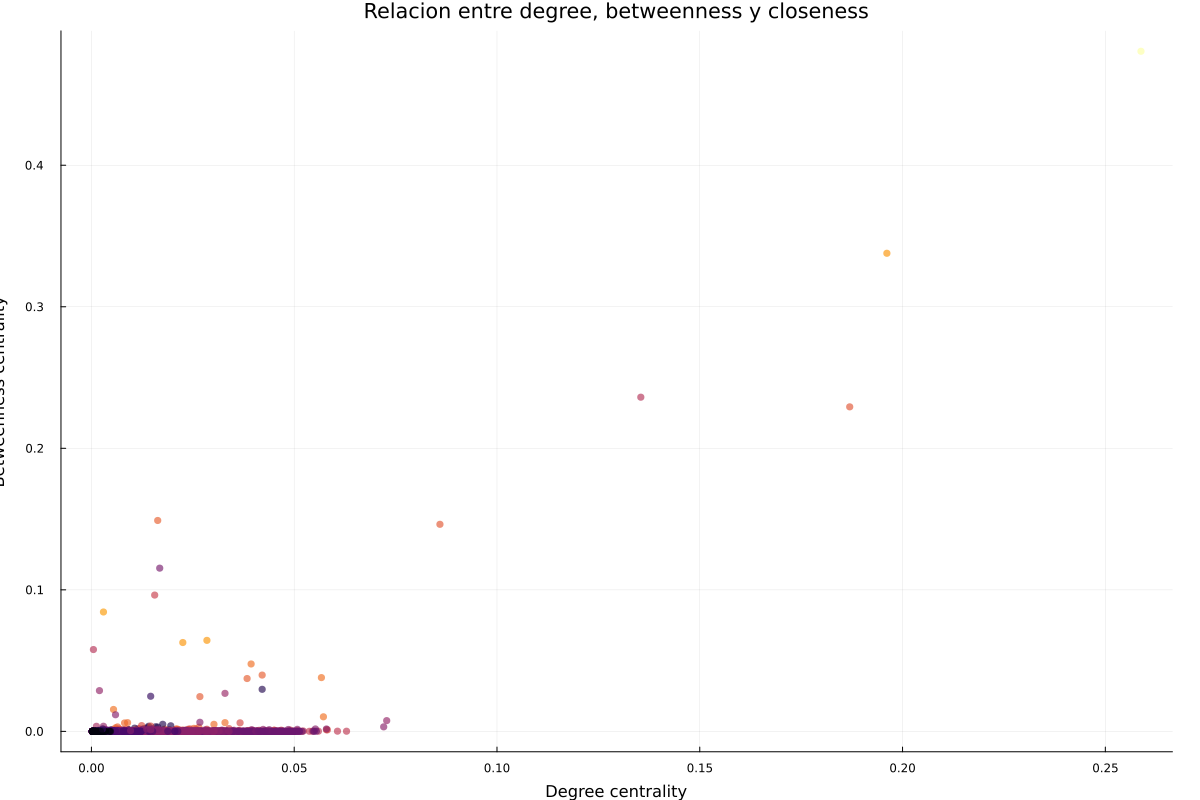
\includegraphics[width=\linewidth]{plots/centrality_relationships.png}
\vspace{0.05cm}
{\tiny Cada punto es un usuario. El color corresponde a closeness y permite comparar las tres metricas a la vez.}
\end{columns}
\end{frame}

\begin{frame}{2b. Incoherencias en el reporte generado con IA}
\begin{columns}[T]
\column{0.56\textwidth}
\scriptsize
\begin{itemize}
    \item \textbf{``Microcomunidades'' sin deteccion formal}: el informe infiere comunidades solo por el valor de clustering, sin ejecutar ningun algoritmo (ej. Louvain).
    \item \textbf{Small-world sin referencia comparativa}: se concluye patron small-world por baja densidad y diametro corto, pero no se compara contra una red aleatoria equivalente.
    \item \textbf{K-core 115 = ``nucleo cohesionado''}: el informe usa ese termino sin definir un umbral que justifique cuando un k-core es alto o bajo para esta red.
    \item \textbf{Componente gigante y 100\% reportados como datos separados}: ambos expresan lo mismo; repetirlos puede inflar la percepcion de solidez de la red.
\end{itemize}
\column{0.44\textwidth}
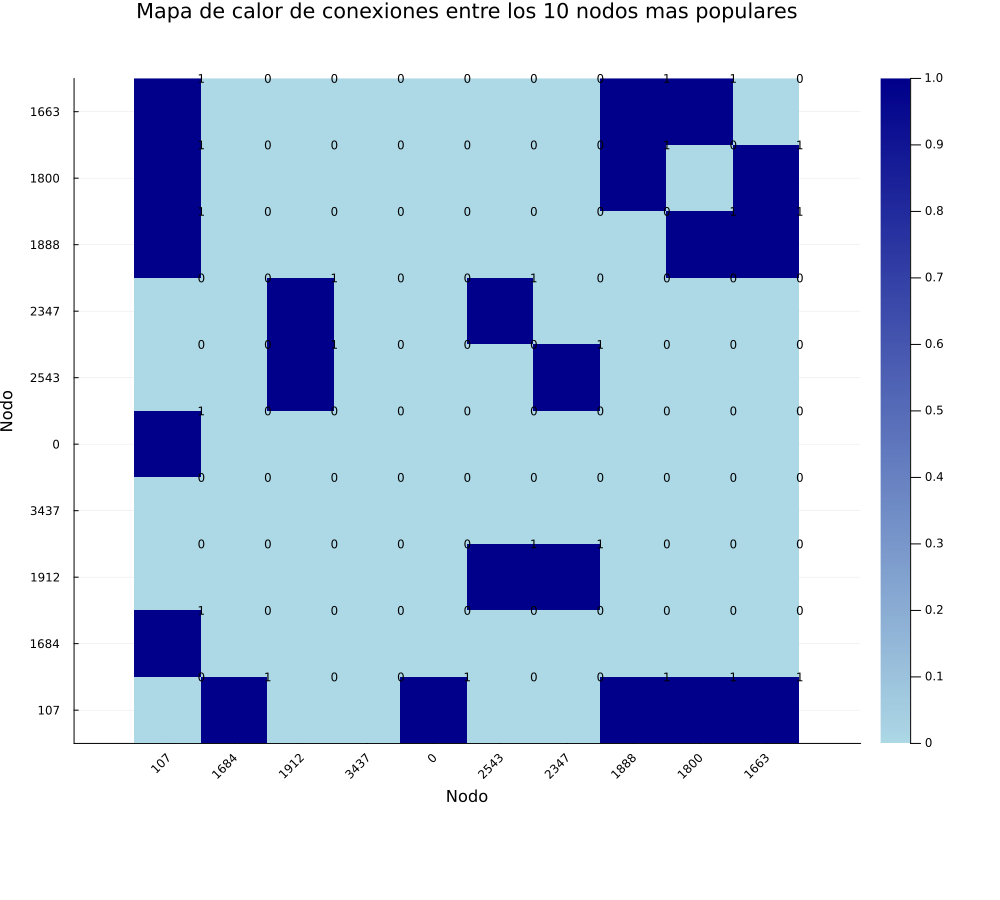
\includegraphics[width=\linewidth]{plots/top10_populares_heatmap.png}
\vspace{0.05cm}
{\tiny Mapa de adyacencia del top 10. Las celdas con valor 1 confirman que los hubs no estan densamente interconectados entre si.}
\end{columns}
\end{frame}

\begin{frame}{3. Metricas mas relevantes para este analisis}
\begin{columns}[T]
\column{0.56\textwidth}
\small
\begin{itemize}
    \item \textbf{Degree (popularidad):} cuantos contactos directos tiene un nodo.
    \item \textbf{Betweenness (puente):} cuanto conecta grupos distintos (control de flujo).
    \item \textbf{Closeness (rapidez):} que tan rapido llega al resto de la red.
    \item \textbf{Clustering y k-core (cohesion):} muestran comunidades fuertes y un nucleo central estable.
\end{itemize}
\vspace{0.2cm}
\textbf{En este informe:} combinar estas metricas evita conclusiones parciales.
\column{0.44\textwidth}
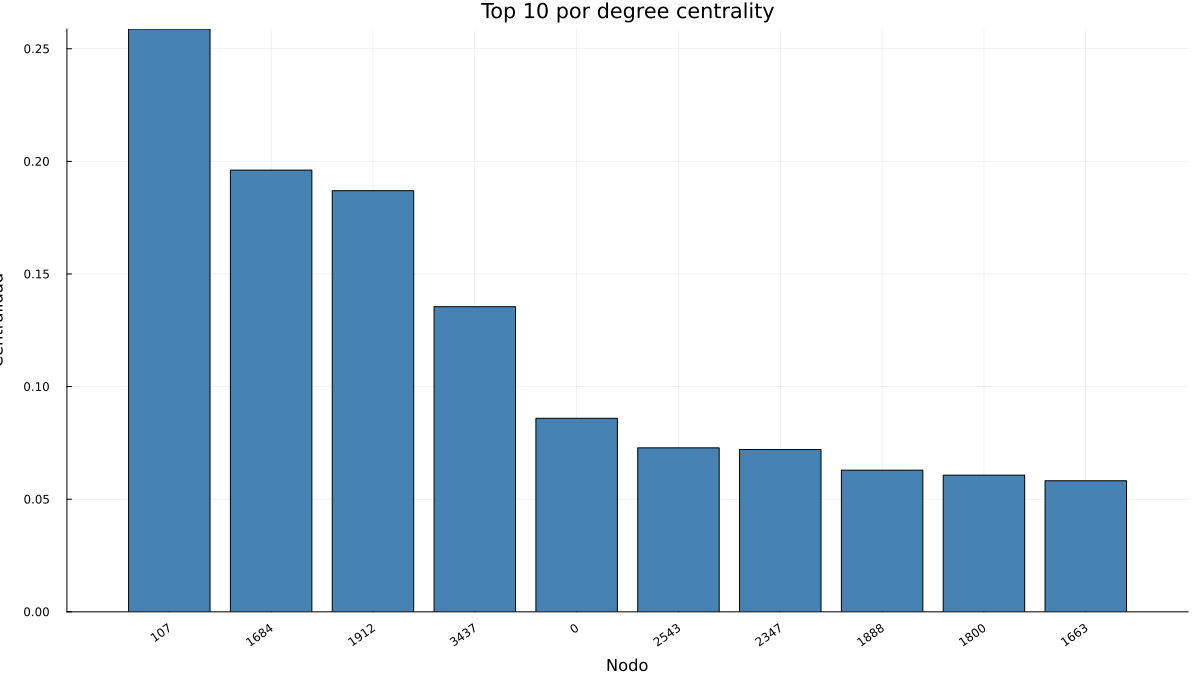
\includegraphics[width=\linewidth]{plots/top_degree.png}
{\tiny Usuarios con mayor numero de conexiones directas.}
\vspace{0.05cm}
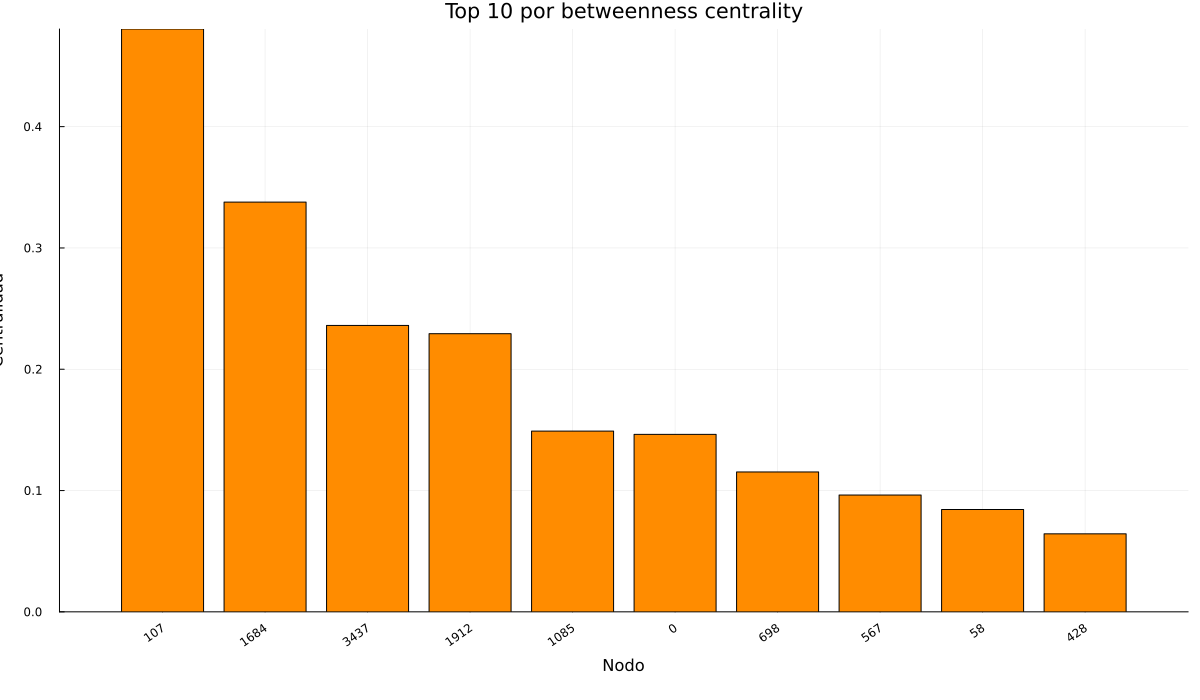
\includegraphics[width=\linewidth]{plots/top_betweenness.png}
{\tiny Nodos que actuan como puentes entre regiones de la red.}
\end{columns}
\end{frame}

\begin{frame}{4. Aplicacion de resultados a un caso real}
\begin{columns}[T]
\column{0.56\textwidth}
\small
\begin{itemize}
    \item \textbf{Caso: campana de salud publica en red social.}
    \item \textbf{Paso 1 (arranque):} publicar con nodos mas populares (top degree) para ganar alcance rapido.
    \item \textbf{Paso 2 (expansion):} usar nodos puente (top betweenness) para entrar a comunidades distintas.
    \item \textbf{Paso 3 (velocidad):} reforzar con nodos de alto closeness para reducir tiempo de difusion.
    \item \textbf{Paso 4 (riesgo):} no depender de un unico hub; repartir mensajes porque el top 10 concentra 2.72\%.
\end{itemize}
\column{0.44\textwidth}
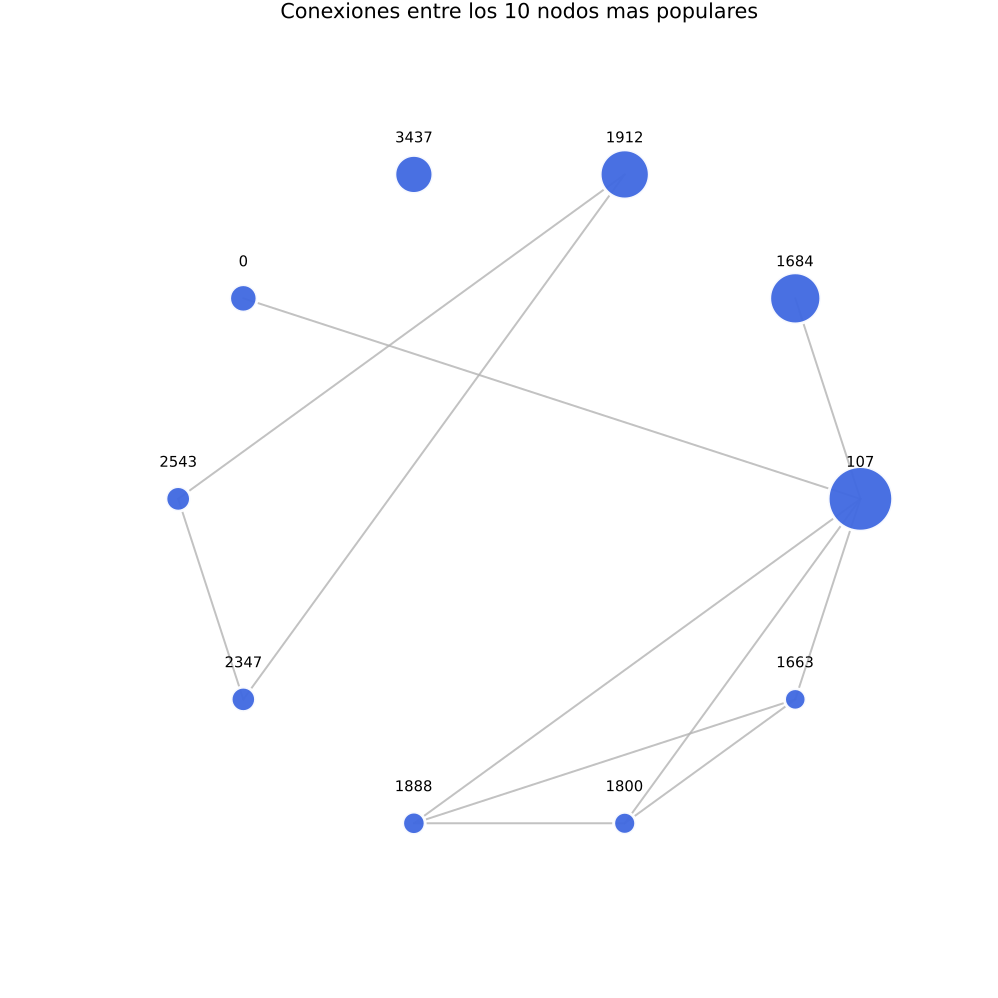
\includegraphics[width=\linewidth]{plots/top10_populares_subgrafo.png}
\vspace{0.05cm}
{\tiny Los 10 hubs del informe y las conexiones entre ellos. Permite ver si se conectan entre si o concentran enlaces hacia la periferia.}
\end{columns}
\end{frame}

\end{document}
